\begin{center}
    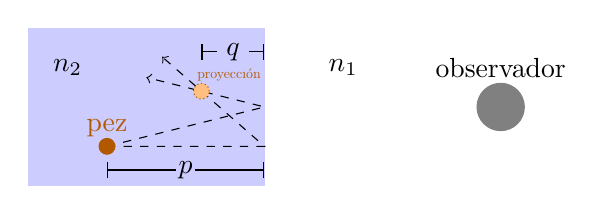
\begin{tikzpicture}
        \filldraw[blue!20] (-2,0) rectangle (1,2);

        \draw[ ->, dashed ] (-1,0.5) -- (1,1) -- (-0.5,1.375);
        \draw[ ->, dashed ] (-1,0.5) -- (1,0.5) -- (-0.3,1.6375);
        \draw[densely dotted, orange!70!black, fill=orange!50] (0.2,1.2) circle (1mm)
        node[yshift=2mm, xshift=3.5mm, scale=0.5] {proyección};

        \filldraw[orange!70!black] (-1,0.5) circle (1mm) node[above] {pez};
        \filldraw[black!50] (4,1) circle (3mm) node[yshift=5mm, color=black] {observador};


        \draw[|-|] (-1, 0.2) -- (1,0.2) node[midway,fill=blue!20,inner sep = 1pt] {$p$};
        \draw[|-|] (0.2, 1.7) -- (1,1.7) node[midway,fill=blue!20] {$q$};

        \draw (-1.5,1.5) node {$n_2$};
        \draw (2,1.5) node {$n_1$};
    \end{tikzpicture}
\end{center}